\documentclass[a4paper,11pt,fleqn]{article}%fleqn pour aligner les equations à gauche
\usepackage{/home/rweye/Documents/Overleaf/Styles/Cours}


\newcommand{\chnum}{Chapitre 14b}
\newcommand{\chtitle}{Bilan radiatif terrestre}
\newcommand{\dtype}{Cours}
  
\begin{document}
	\maketitle
\section{Loi de Stefan-Boltzmann}
Tout corps à température $T$ émet un rayonnement électromagnétique. La loi de Stefan-Bortzmann permet d'établir une relation entre le flux thermique surfacique émis $\phi$ et la température $T$ :
$$\phi = \sigma \cdot T^4$$
Avec : $\phi$ le flux thermique surfacique émis par un corps (\unit{\watt\per\meter\squared})\\
$\sigma$ la constante de Stefan-Boltzmann égale à $\sigma = \SI{5,67E-8}{W m^{-2} K^{-4}}$\\
$T$ la température du corps (\unit{\kelvin})

\section{Bilan radiatif terrestre}
Le rayonnement solaire parvenant jusqu'à la Terre est sa source principale d'énergie thermique. Comme la température moyenne de la surface de la Terre est stable au fil des ans, cela signifie que la surface reçoit en moyenne autant d'énergie qu'elle en émet vers l'espace par son propre rayonnement.\\
La Terre reçoit un rayonnement solaire dont le flux thermique surfacique moyen est de l'ordre de $\phi_s =\SI{340}{\watt\per\meter\squared}$. Environ $\alpha = \SI{30}{\percent}$ de ce rayonnement est réfléchi sans être absorbé par l'atmosphère : cette proportion est appelée \textbf{albédo}.\\
Plus l'albédo est élevé, plus le rayonnement solaire est réfléchi et moins la surface de la Terre reçoit d'énergie thermique.\\
Si une partie du rayonnement émis par la Terre n'était pas absorbée par l'atmosphère (principalement dans le domaine des infrarouges), la température à la surface serait d'environ \SI{-18}{\celsius}. Cette absorption essentiellement due à la présence d'eau \ce{H2O} et de dioxyde de carbone \ce{CO2} dans l'atmosphère s'appelle \textbf{l'effet de serre}.\\
Cet effet de serre naturel permet à la surface de la Terre de récupérer une partie de l'énergie qu'elle rayonne, contribuant ainsi à son réchauffement jusqu'à une température moyenne de \SI{15}{\celsius}.

\newpage
\section{Activité : Température terrestre moyenne}
Le rayonnement solaire est la principale source d'énergie de la Terre. Cette énergie est reçue sous forme de radiations ultraviolettes, visibles et infrarouges. La Terre, du fait de la température de sa surface, perd de l'énergie sous forme de radiation infrarouges émises vers l'espace.

\begin{enumerate}
	\item \begin{enumerate}
		\item En utilisant la loi de Stefan-Boltzmann, déterminer la puissance solaire surfacique $\mathcal{p}_S$ émise au niveau de la surface du Soleil considéré comme un corps noir.
		\item Montrer que la puissance solaire surfacique $\mathcal{p}'_S$ à la distance $D$ entre la Terre et le Soleil est \SI{1,36E3}{\watt\per\meter\squared}.
		\item Exprimer la puissance solaire incidente interceptée par la Terre $\mathcal{P}_T$.
		\item  En déduire la puissance solaire incidente surfacique $\mathcal{p}_T$ reçue en moyenne par le système \{Terre et atmosphère\}.
	\end{enumerate}
	\item \begin{enumerate}
		\item Évaluer la puissance solaire surfacique moyenne $\mathcal{p}_{T(abs)}$ absorbée par le système \{Terre et atmosphère\}.
		\item On considère que le système \{Terre et atmosphère\} réémet toute la puissance qu'il reçoit. En déduire la température moyenne théorique du système.
		\item Retrouver que la température terrestre moyenne théorique au niveau du sol en absence d'albédo est voisine de \SI{5}{\celsius}.
		\item En réalité, la température terrestre moyenne au niveau du sol est voisine de \SI{15}{\celsius}. À partir du schéma C, proposer une explication à l'écart entre cette température et celle calculée en 2b.
	\end{enumerate}
	\item Proposer une explication scientifique aux observations décrites dans le document D.
	\item De quoi la température moyenne de la surface terrestre dépend-elle ?
\end{enumerate}

\begin{figure}[h!]
	\begin{minipage}{.48\textwidth}
	\caption{Puissance solaire surfacique reçue par le système \{Terre et atmosphère\}}
	Le rayonnement solaire qui se propage dans le vide n'est pas absorbé. À une distance $D$ du Soleil, la puissance totale qu'il émet se répartit sur une sphère de rayon $D$. On peut alors déterminer la puissance solaire surfacique à cette distance.
	\begin{center}
	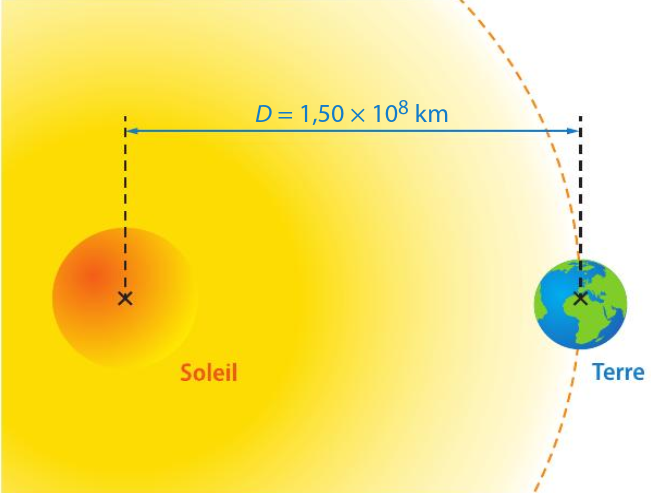
\includegraphics[width=\linewidth]{Ressources/TSPE_C14_Act3_Fig1.png}
	\end{center}
	\end{minipage} \hspace{1em}
	\begin{minipage}{.48\textwidth}
	\caption{Puissance solaire reçue par le système \{Terre et atmosphère\}}
	Au niveau de la Terre, la puissance solaire surfacique d'étale sur un disque de rayon $R_T$.\\
	Comme la Terre tourne sur elle-même, cette puissance se répartit sur l'ensemble de la surface du globe terrestre.
	\begin{center}
	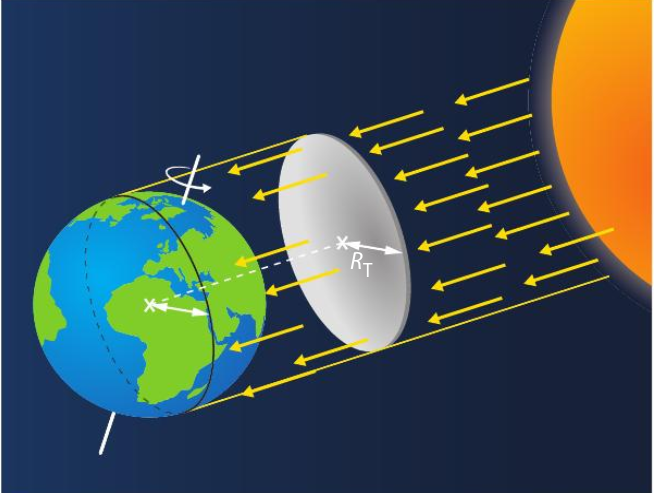
\includegraphics[width=\linewidth]{Ressources/TSPE_C14_Act3_Fig2.png}
	\end{center}
	\end{minipage}
\end{figure}


\begin{figure}[h!]
	\begin{center}
	\caption{Bilan radiatif du système \{Terre et atmosphère\}}
	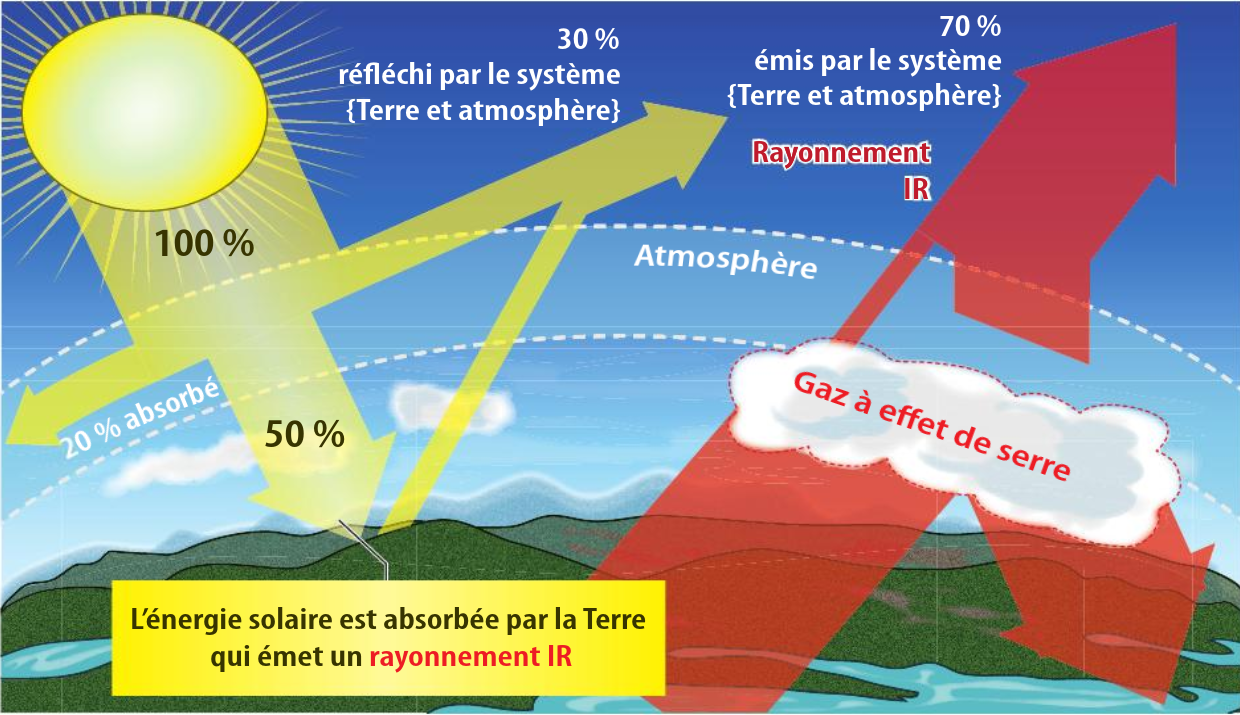
\includegraphics[width=.5\linewidth]{Ressources/TSPE_C14_Act3_Fig3.png}
	\end{center}
\end{figure}


\begin{figure}[h!]
	\caption{Choix réfléchi de couleurs}
	\begin{multicols}{2}
	\begin{center}
		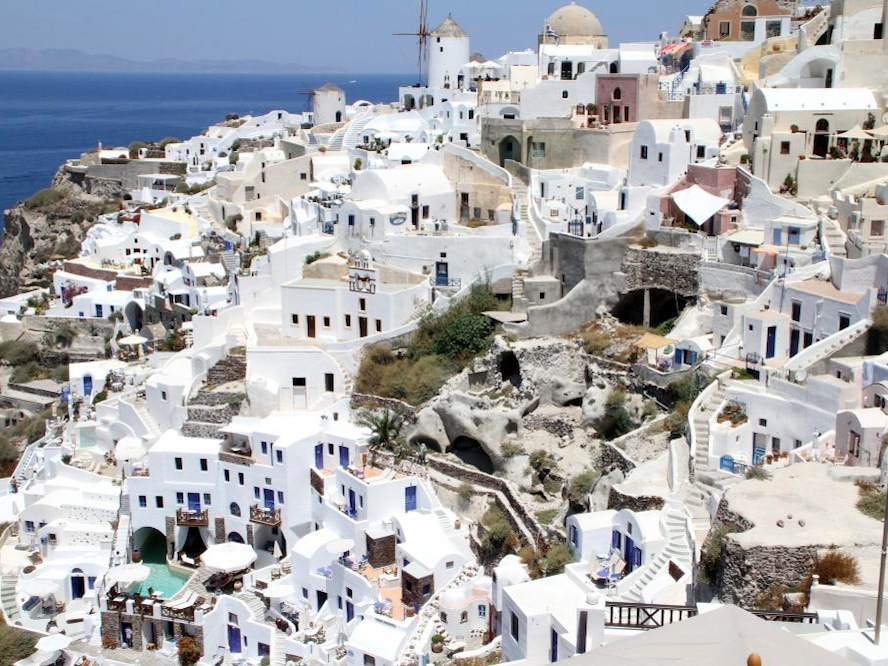
\includegraphics[width=.7\linewidth]{Ressources/VillageGrece.jpg}
	\end{center}
	\begin{scriptsize}
		Recouvrir les murs de chaux blanche, comme en Grèce, permet de mieux supporter les épisodes de forte chaleur.
	\end{scriptsize}
	\columnbreak
	
	\textbf{Données :}
	\begin{itemize*}
		\item Rayon du Soleil : $R_S = \SI{6,96E8}{m}$
		\item Rayon de la Terre : $R_T = \SI{6,37E6}{m}$
		\item Surface d'une sphère de rayon $R$ : $S = 4\pi \times R^2$
		\item Température moyenne de surface du Soleil : $T = \SI{5778}{K}$
		\item Albédo du système \{Terre et atmosphère\} = $\alpha \approx 0,30$
	\end{itemize*}
	\end{multicols}
\end{figure}

\begin{figure}[h!]
\caption{Complément scientifique}
\begin{multicols}{2}
\textbf{Puissance surfacique}\\
La puissance surfacique $\mathcal{p}$ est la puissance par unité de surface.
$$\mathcal{p} = \dfrac{\mathcal{P}}{S}$$

\textbf{Loi de Stefan-Boltzmann}\\
Un corps noir de température constante réémet tout le rayonnement qu'il absorbe.\\
La puissance surfacique $\mathcal{p}$ émise par un corps noir est lié à sa température par la relation :
$$\mathcal{p} = \sigma \cdot T^4$$
avec $\sigma = \SI{5,67E-8}{W m^{-2} K^{-4}}$, la constante de Stefan-Boltzmann.

\columnbreak
\textbf{Albédo}
\begin{multicols}{2}
L'albédo $\alpha$  d'une surface est une grandeur sans unité qui caractérise son aptitude à renvoyer par diffusion et/ou réflexion le rayonnement qui lui parvient.
$$ \alpha = \dfrac{|\mathcal{P_r}|}{\mathcal{P} = \dfrac{|\mathcal{p}_r|}{\mathcal{p}_i}}$$
avec $\mathcal{P}_r$ la puissance renvoyée par la surface.

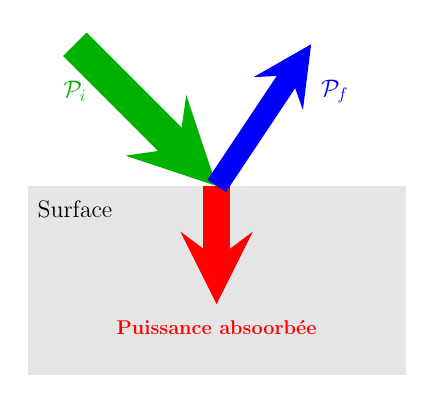
\begin{tikzpicture}[scale=.6, transform shape]
	\fill[gray!20] (0,0) rectangle (8,4);
	\draw[red,line width = 10pt, -stealth] (4,4) to (4,1.5);
	\draw[green!70!black,line width = 12pt, -stealth] (1,7) to (4,4);
	\draw[blue,line width = 8pt, -stealth] (4,4) to (6,7);
	
	\node[red] (Pa) at (4,1){\large \textbf{Puissance absoorbée}};
	\node[green!70!black] (Pi) at (1,6){\Large {$\mathcal{P}_i$}};
	\node[blue] (Pf) at (6.5,6){\Large {$\mathcal{P}_f$}};
	\node (S) at (1,3.5){\Large Surface};
\end{tikzpicture}
\end{multicols}

\textbf{Conversion des températures}
$$T=\theta + \num{273,15}$$
\end{multicols}
\end{figure}


\end{document}